\documentclass[10pt, twocolumn]{ctexart}

\usepackage{stfloats}
\usepackage[left=2.5cm, right=2.5cm, top=2.5cm, bottom=2.5cm]{geometry}
\usepackage{url}
\usepackage{xtab, booktabs}
\usepackage{mathptmx}
\usepackage{amsmath}
\usepackage{xcolor}
\usepackage{hyperref}
\usepackage{subfigure}
\usepackage{graphicx}
\graphicspath{{images/}}
\usepackage[backend=biber, style=gb7714-2015, hyperref=auto]{biblatex}
\addbibresource{reference.bib}


\newcommand\rr[1]{\textcolor{red}{#1}}


\title{通过快速搜索和寻找密度峰进行聚类\footnote{翻译自\citeauthor{Rodriguez2014}(\citeyear{Rodriguez2014})一文. }}
\author{Alex Rodriguez \and Alessandro Laio}
\date{}


\begin{document}

    \begin{titlepage}
        \maketitle
        \begin{abstract}
    时域速度和\rr{正常时差参数(moveout parameters)}可以直接从\rr{同相轴局部斜率(local event slopes)}中获得, 而\rr{同相轴局部斜率}是基于叠前地震道集估计出来的. 在实际应用中, 估计出的局部斜率总是有一定的误差, 特别是在信噪比较低的情况下. 因此, 地下速度信息可能隐藏在速度和其他\rr{正常时差参数}所决定的图像中. 我们开发了一种加速聚类算法, 可以在事先不知道聚类中心数量的情况下寻找聚类中心. 首先, 实施\rr{平面波解构(plane-wave destruction)}来估计\rr{同相轴局部斜率}. 对于地震道集中的每一个样本, 我们根据\rr{同相轴局部斜率}获得速度的估计和它在图像域中的位置. 这些被映射到新的空间中的点展现出了不同类的结构. 我们用混合分布模型来对这些点进行建模. 然后, 对混合模型的聚类中心进行确定, 这些聚类中心就对应着主要地下构造的极大似然速度. 利用估算的速度的不确定约束来选择对应的反射中心. 最后, 对聚类后的采样不均匀的结速度进行插值, 在规则格网上建立高效的速度模型. 在人工合成数据和实际数据上实施该算法, 我们确定了所提出它可以给出精度相对较高的叠加速度模型和时偏移速度模型. 
\end{abstract}
    \end{titlepage}


    \section{简介}
速度估计是地震反问题中的一项重要任务. 宏模型的建立通常是从用不同的动校正速度对CMP道集进行扫描开始的. 手动选取速度谱上的能量峰值点是一个十分费力的过程, 需要有经验的专业的数据处理员才能完成这个任务. 在过去的几十年里, 人们采取了各种方法来完成自动的速度分析. (\cite{Toldi1989})描述了一种最早的自动速度分析算法, 其中速度模型是由可能的区间速度表示的. 沿着动校正曲线将\rr{堆积功率(stacking power)}最大化, 从而获得最佳的速度模型. \rr{相似谱(semblance spectra)}上的自动速度选取问题也可以看作是一个射线跟踪问题. 将相似谱上的能量(\cite{Fomel2009})作为慢度, 则相似谱顶部到底部具有最小移动时间的射线路径就对应一个最佳的选取速度. 为了克服在CMP道集上的速度分析中的反射点分散问题, 可以通过包括各向异性在内的速度延续来建立时偏移速度模型(\cite{Adler2002,Fomel2003,Alkhalifah2011,Burnett2011}). 还有一种叫作\rr{图像波传播(image wave propagation)}的类似的方法(\cite{Schleicher2008}). 不同速度的重复时偏移(\cite{Yilmaz2001a})也是一种替代方法. 

另一种方法是使用\rr{同相轴局部斜率}. 在地震道集上接收到的的同相轴局部斜率包含了珍贵的地下信息. 动校正速度(NMO)和时偏移速度可以直接从同相轴局部斜率中得出. (\cite{Ottolini1983})提出了与速度无关的同相轴局部斜率成像. (\cite{Fomel2007})和(\cite{Cooke2009})表明, 利用叠前反射数据估计的同相轴局部斜率可以完成几乎所有常见的时域成像任务和速度估计. 地震数据或地震图像中包含的同相轴局部斜率和其他局部时差属性也可用于深度域上的速度模型反演, 如立体成像(\cite{Billette1998,Lambare2008})等. 

同相轴局部斜率估计的好坏决定了基于同相轴局部斜率的成像和反演结果. \rr{局部倾斜叠加}(\cite{Ottolini1983})是提取同相轴局部斜率的标准工具之一. 希尔伯特变换(\cite{Barnes1996,Cooke2009,Zhang2013,Wang2015})也可以用来得到等于同相轴局部斜率的相位移. 另一种具有鲁棒性的斜率估计算法是\rr{平面波解构(plane-wave destruction)}(PWD)(\cite{Fomel2002, Schleicher2009}). PWD通过平面波来逼近局部波场. 通过最大限度上扁平化分数延迟滤波器, Chen等人(\cite{Chen2013,Chen2013a})进一步加速了PWD方法, 并使其适用于陡峭层. 由于估计的同相轴局部斜率总是受到噪声和干扰事件的影响而退化, 所以直接映射算子可能会导致成像部分受到高频振荡的污染, 从同相轴局部斜率得到的速度对噪声很敏感. 虽然图像扭曲的速度图可以得到与同相轴局部斜率相关的时域速度, (\cite{Fomel2007})但当地震道集中包含多个散射或多路径事件时, 速度图就会变得相当复杂. 速度图上的能量可以作为慢度, 从而通过求解初至射线追踪问题来进行自动速度选取. (\cite{Cooke2009})在速度图上使用静音和平均滤波器来抑制多路径事件. 

本文提出了一种基于从同相轴局部斜率映射来的局部属性聚类的时域速度自动估计方法. 局部属性由一个混合分布模型来表示. 混合分布模型的聚类中心对应于主要地下构造的极大似然速度. 这些聚类中心对由噪声、干扰事件和多路径事件引起的同相轴局部斜率退化具有鲁棒性. 我们开发了一种加速聚类算法, 从而高效率地找到聚类中心. 在聚类后的不均匀采样中心上进行最小二乘插值, 建立规则格网上的高效速度模型. 通过在人工合成和实际数据上实施, 我们评估了所提出的算法的性能, 并证实了它符合我们理论上的预期. 


    \begin{figure*}
    \centering
    \subfigure[使用随机噪声合成的人工CMP道集. \label{fig:1a}]{
        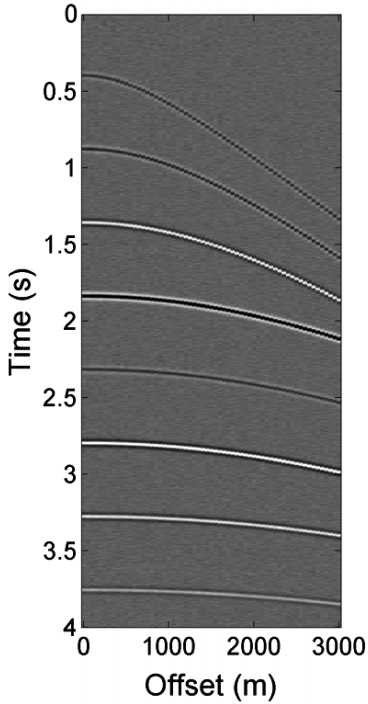
\includegraphics[scale=.35]{1a.png}
    }\ 
    \subfigure[使用PWD来估计斜率. \label{fig:1b}]{
        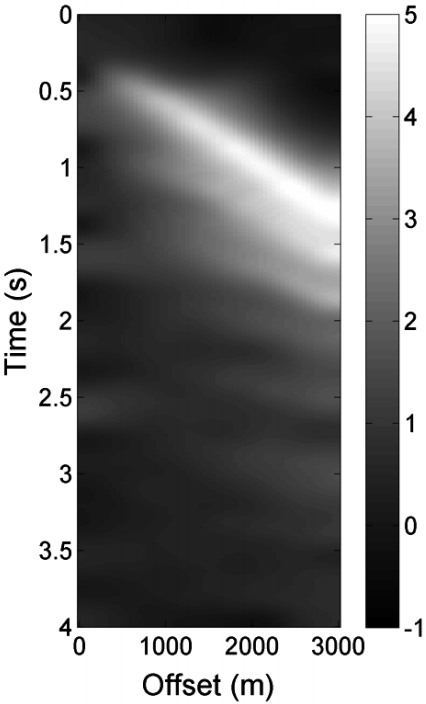
\includegraphics[scale=.35]{1b.png}
    }\ 
    \subfigure[从局部属性计算局部斜率的结果. \label{fig:1c}]{
        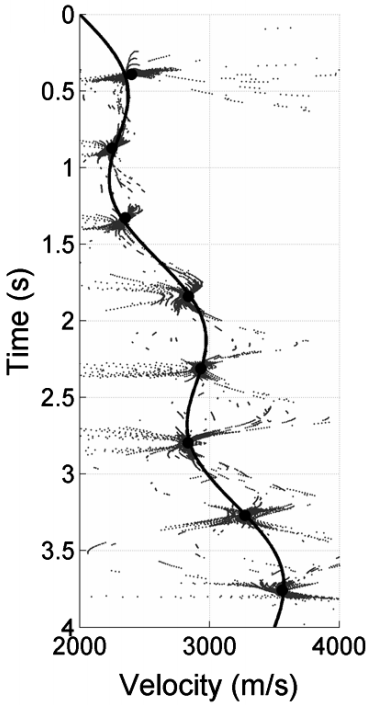
\includegraphics[scale=.35]{1c.png}
    }
    \caption{随机噪声为10dB的人工数据示例. \ref{sub@fig:1c} 中, 灰色数据点是映射后的数据, 黑色圆圈是聚类中心, 黑色曲线表示真实速度. 
    }
\end{figure*}
\begin{figure*}
    \centering
    \subfigure[使用随机噪声的人工合成 CMP 道集. \label{fig:2a}]{
        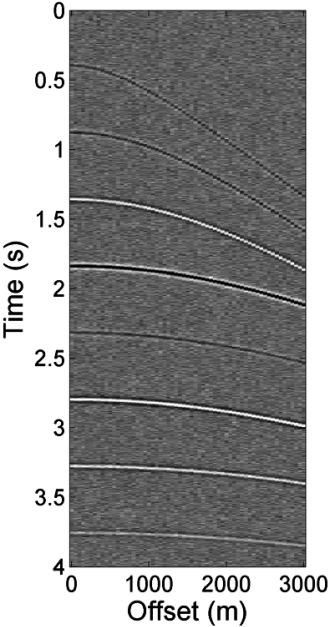
\includegraphics[scale=.36]{2a.png}
    }\ 
    \subfigure[使用 PWD 估计斜率. \label{fig:2b}]{
        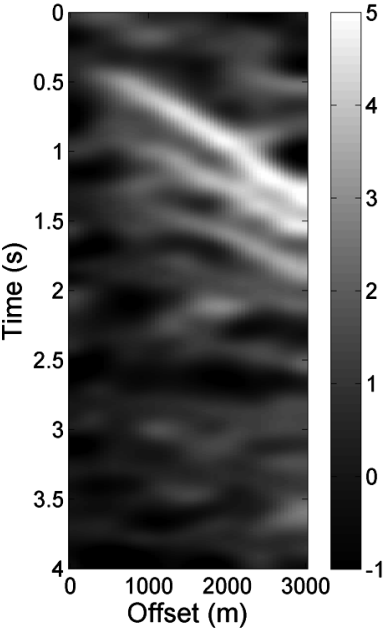
\includegraphics[scale=.36]{2b.png}
    }\ 
    \subfigure[从局部属性映射到局部斜率的结果. \label{fig:2c}]{
        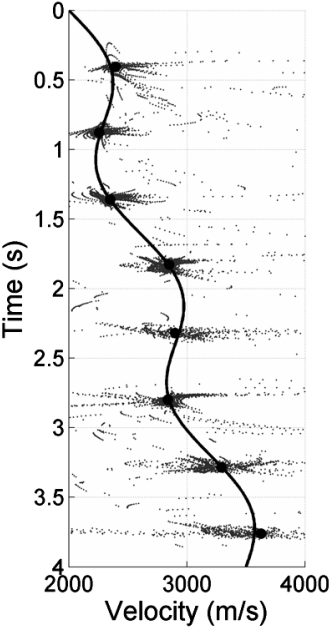
\includegraphics[scale=.36]{2c.png}
    }
    \caption{加入0dB随机噪声的人工数据示例. }
\end{figure*}
\section{理论}
在本节中, 我们通过混合分布模型来说明模型的建立过程. 其中加速密度聚类算法是通过一些计算和分析给出的, 叠加速度和迭前时偏移速度模型是通过对聚类中心进行插值估计出来的. 
\subsection{混合分布模型}
局部同相轴斜率包含地下反射的几何和速度信息, 有了估计出的局部同相轴斜率, 我们可以用简单的一对一映射算子在时域中生成图像. 从反射时差的经典双曲假设开始: 
\begin{equation}
    t^2(h)=\tau_0^2+\frac{h^2}{V_{\mathrm{NMO}}^2(\tau_0)}
\end{equation}
其中$\tau_0$为双向零偏距走时, $t(h)$代表偏移量$h$处记录的双向走时, $V_{\mathrm{NMO}}(\tau_0)$为叠加速度. 我们将$t(h)$相对于$h$的导数记为$p_h$(走时斜率):
\begin{equation}
    p_{h}(t, h)=\frac{d t}{d h}=\frac{h}{t V_{\mathrm{NMO}}^{2}\left(\tau_{0}\right)}
\end{equation}

通过上述两个方程, 叠加速度$V_{\mathrm{NMO}}(\tau_0)$和零偏距走时$\tau_0$可以被有效的表示出来(\cite{Ottolini1983, Fomel2007}), 即: 
\begin{equation}
    V_{\mathrm{NMO}}\left(\tau_{0}\right)=\sqrt{\frac{h}{t p_{h}(t, h)}}
    \label{equ:3}
\end{equation}
和
\begin{equation}
    \tau_{0}=\sqrt{t^{2}-t p_{h}(t, h) h}
    \label{equ:4}
\end{equation}

为了在每个CMP道集上得到一个稳健的局部同相轴斜率估计$p_h$, 我们采用了PWD(\cite{Fomel2002, Chen2013})算法. 在具体应用时可以针对不同的问题将斜率估计算法替换为其他算法. $\{t,h\}$空间上的单个CMP道集数据点可以通过方程(\ref{equ:3})和(\ref{equ:4})映射到零偏距走时和叠加速度空间$\{\tau_0,V_{\mathrm{NMO}}\}$中, 但在偏移点的附近, 局部同相轴斜率会接近零, 因此, 我们不使用零偏移点附近的数据. 另外, 与使用通过图像扭曲的速度图(\cite{Fomel2007})不同的是, 我们不再使用数据点的振幅, 而是将数据点以相等的权重映射到新的空间中. 对于实际数据的应用, 可以用从估计的斜率中得到的局部相干性来分配每个数据的权重(\cite{Zhang2013}). 图~\ref{fig:1a} 是使用8个收集器的在速度平滑变化的介质中的简单实验. CMP道集的Ricker子波峰值频率为 20 Hz, 接收器的间隔为 50 m, 电缆总长度为 3 km, 时间间隔为4 ms, 总时间为 4 s, 该图是将速度从从 2.0 km∕s开始应用逆动校正获得的. 图~\ref{fig:1b} 描述了PWD估计出的局部同相轴斜率, 可以看出, 估计出的局部同相轴斜率相当平稳. 图~\ref{fig:1c} 显示了数据点映射到$\{\tau_0,V_{\mathrm{NMO}}\}$空间后的分布. 

需要注意的是, 新空间中的数据点有成簇的性质. 鉴于反射时差的双曲假设可以完全描述反射事件的过程, 并且能完美估计局部同相轴斜率, 因此, 新空间中的数据点应该对应一次相同位置上的反射事件. 但在面对实际数据时, 双曲假设并不能完全描述非平面反射体, 因此, 估计出的斜率永远会有偏差, 表现为一个反射事件被映射成一簇. 假定双曲假设和斜率估计算法的误差遵循高斯分布, 那么, 一次反射数据的计算结果可以用一个高斯分布来表示, 其期望值为极大似然估计. 对于多于一次反射的情况, 我们也可以直观的引入高斯混合模型, 作为高斯分布的简单线性叠加, 高斯混合模型可以表示更加复杂的密度模型(\cite{Bishop2006}), 其表示如下: 
\begin{equation}
    P(\mathbf{x})=\sum_{k=1}^{K} a_{k} N_{k}\left(\mathbf{x} \mid \mu_{k}, \sigma_{k}\right)
\end{equation}
其中, $x$为计算得到的数据点在新空间中的位置, $N_{k}\left(\mathbf{x} \mid \mu_{k}, \sigma_{k}\right)$为高斯分布, $x$的期望为$\mu_k$, 标准差为$\sigma_k$, $K$代表单个高斯分布的总数量, $a_k$为混合系数, $P(x)$是联合分布$P(x|x\in N_k)$对所有可能的状态$P(x\in N_k)$的求和, 即
\begin{equation}
    P(\mathbf{x})=\sum_{k=1}^{K} P\left(\mathbf{x} \in N_{k}\right) P\left(\mathbf{x} \mid \mathbf{x} \in N_{k}\right)
\end{equation}
其中$P(x\in N_k)$等价于混合系数$a_k$. 通过寻找这$K$个聚类中心, 可以有效地计算出每个高斯分布的期望值$\mu_k$. 

在图~\ref{fig:1c} 中, 黑色圆圈代表聚类中心, 它给出了速度的极大似然解, 黑色曲线为真实的NMO速度. 可以看出, 所有的聚类中心都落在了真实的NMO速度的路径上. 聚类中心的数量为8个, 等于反射体的数量. 因此, 混合分布模型可以有效地解决计算从局部同相轴斜率映射的速度值的极大似然解的问题. 

但同样的, 估计出的局部同相轴斜率的质量会因为噪声和干扰而降低, 图~\ref{fig:2a} 显示了与图~\ref{fig:1a} 中相同的CMP道集, 但添加了更强的信噪比为0dB的随机噪声. 在这种情况下, 信号的功率等于随机高斯噪声的功率. 图~\ref{fig:2b} 展示了PWD估计出的局部同相轴斜率, 尽管在PWD之前已经使用了带通滤波器来过滤噪声, 但估计出的局部同相轴斜率仍受到了强噪声的影响. 图~\ref{fig:2c} 显示了在$\{\tau_0,V_{\mathrm{NMO}}\}$空间中的新数据点, 直接映射算子给出了被高频振荡污染的部分. 在图~\ref{fig:2c} 中, 黑色圆圈代表聚类中心, 黑色实心曲线是真实的NMO速度. 可以看出, 此时所有的聚类中心仍然与真实NMO速度的路径相吻合, 这证实了聚类中心对局部同相轴斜率的估计是稳健的. 
\subsection{加速密度聚类}
在所有用于寻找聚类中心的算法中, k-means可能是应用最广泛的, 为了实施k-means算法, 需要提前知道聚类中心的数量, 但这一先验信息通常难以确定(\cite{Hamerly2004}). 但好在\citeauthor{Wang2012}(\citeyear{Wang2012})实现了层次聚类和划分, 以便在储层表征中得到正确的聚类中心数量. 另一方面, 通过带分割和合并的k-means方法(\cite{Muhr2009}), 我们可以在合理的运行时间内选取出准确的聚类中心数量. \citeauthor{Lu2014}(\citeyear{Lu2014})就应用了类似的策略来定位浅水中的衍射地震噪声. 另外, 在k-means中, 数据点总是被分配到距离最近的中心, 虽然我们可以用各种距离将其拓展, 但k-means还是几乎不能检测到非球形簇. 

密度聚类(\cite{Rodriguez2014})则更容易应对更一般的数据分布情况, 聚类簇数也更容易确定. 在密度聚类中, 聚类中心被描述为为密度相对高于相邻点, 而且与其他密度较大的中心点距离较大的点. 对于每个数据点$i$, 其局部密度$\rho_i$和其与密度较高的点的最小距离$\sigma_i$是密度聚类中的两个十分重要的参数. 简单的$\rho_i$定义为:
\begin{equation}
    \rho_{i}=\sum_{j} \lambda\left(d_{i j}-d_{c}\right)
\end{equation}
其中, $d_{ij}$为数据点$i$与数据点$j$之间的距离, $d_c$为截止距离, 如果$d_{ij}-d_c<0$, 则$λ = 1$, 否则$λ = 0$. 该算法仅对不同数据点的$\rho_i$敏感, 这意味着其结果对参数于$d_c$是稳健的(\cite{Rodriguez2014}). 而一个数据点到密度较高的点的最小距离$\sigma_i$为: 
\begin{equation}
    \delta_{i}=\min _{j: \rho_{j}>\rho_{i}}\left(d_{i j}\right)
\end{equation}

对于密度最大的点, $\sigma_i$取值为$\max_j(d_{ij})$. 根据$\sigma_i$的定义, 我们可以得出$\sigma_i$只有在全局或局部最大值时才相对较大的. 然后选取局部密度$\rho_i$相对较大、最小距离$\sigma_i$相对较大的点作为聚类中心. 在实际应用中, 我们可以通过$\beta$的快速变化来确定中心, 即$\beta$是$\rho$和$\sigma$的乘积. 确定聚类中心后, 按照局部密度最高到最低的顺序对数据点进行分配. 数据点总是被分配到离其最近的局部密度较高的那一类中. 总的来说, 密度聚类对$N$个数据点的计算复杂度为$O(N^2)$, 详细复杂度分析见附录~\ref{Appendix:A}. 即使对于单个CMP道集, 在典型的1000个时间样本和100个源-接收器对的情况下, 也可能有105个数据点. 这使得密度聚类算法在实际数据应用中不太合适. 

在模式识别中, 输入数据的分布可能是高度折叠、弯曲或扭曲的, 瑞士卷数据集(\cite{Tenenbaum2000})就是这样一类非线性流形. 在大多数地震数据中, 数据点呈现出的结构都是线性的. 因此, 可以用高斯或类似高斯的分布来逼近数据点的真实分布, 所以我们提出了一种基于直方图函数的加速密度聚类算法. 在统计学中, 直方图是数据分布的一种表示, 在密度聚类中所需要的局部密度由直方图函数来近似表示. 我们应用二维直方图分析方法(\cite{Gonzalez2002,Zhang2015})对计算得到的零偏距时间和叠加速度进行分析, 得到局部密度的估计: 
\begin{equation}
    \rho=H(l_1,l_2)=m(l_1,l_2)
\end{equation}
其中, $l_1$和$l_2$分别代表零偏距时间和叠加速度, $H(l_1,l_2)$是二维直方图函数, $m(l_1,l_2)$是零偏距时间和叠加速度对在同一个组距内的的个数, 这个组距用$l_1,l_2$所代表. 直方图可以用估计出的同相轴局部斜率的相干性来加权, 以保证稳健性, 因为相干性是映射属性可靠性的自然度量. 
\begin{figure}[htb]
    \centering
    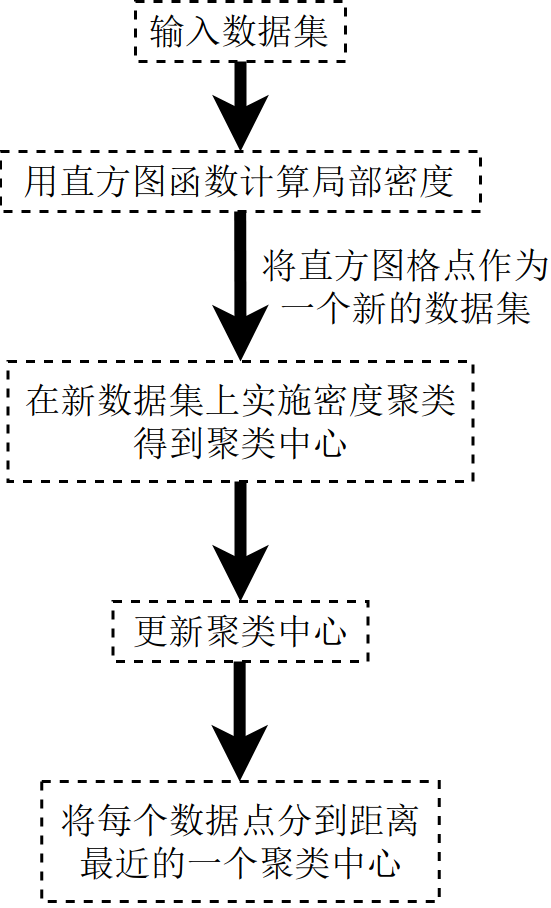
\includegraphics[scale=.2]{3.png}
    \caption{加速密度聚类算法流程图. \label{fig:3}}
\end{figure}

加速密度聚类算法的流程图如图~\ref{fig:3} 所示. 为了证明加速密度算法的性能, 我们将其应用于``S"数据集(\cite{Fraenti2006}), 
\begin{figure}[htb]
    \centering
    \subfigure[``S"型数据集. \label{fig:4a}]{
        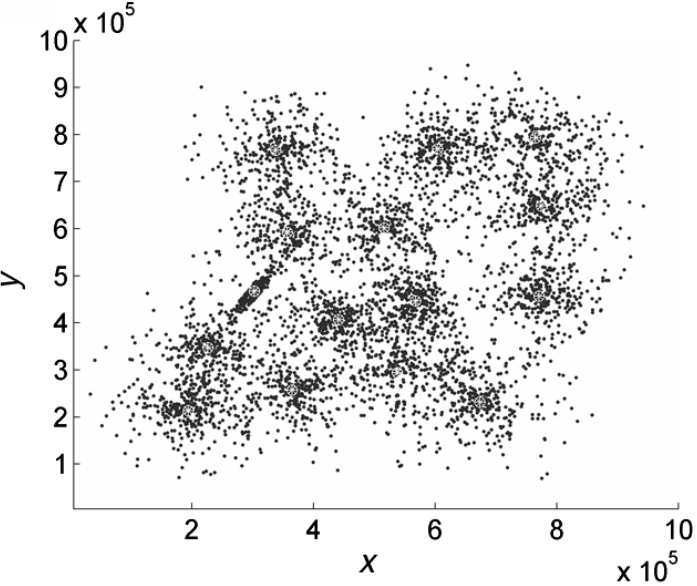
\includegraphics[scale=.15]{4a.png}
    }
    \subfigure[由直方图函数计算出的局部密度. \label{fig:4b}]{
        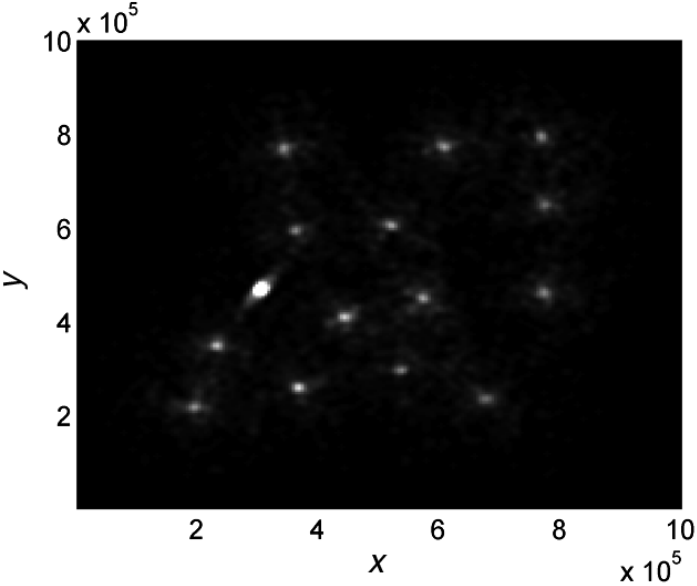
\includegraphics[scale=.15]{4b.png}
    }\\
    \subfigure[直方图上格点的局部密度和最小距离. \label{fig:4c}]{
        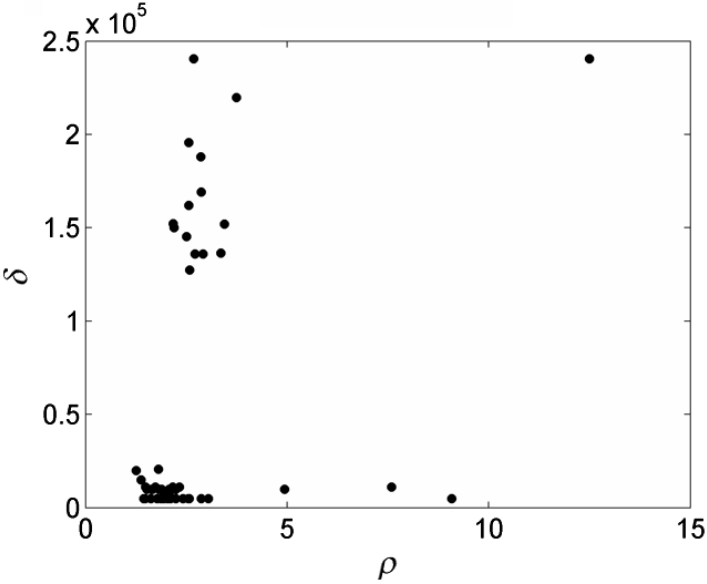
\includegraphics[scale=.15]{4c.png}
    }
    \subfigure[排序后的结果. \label{fig:4d}]{
        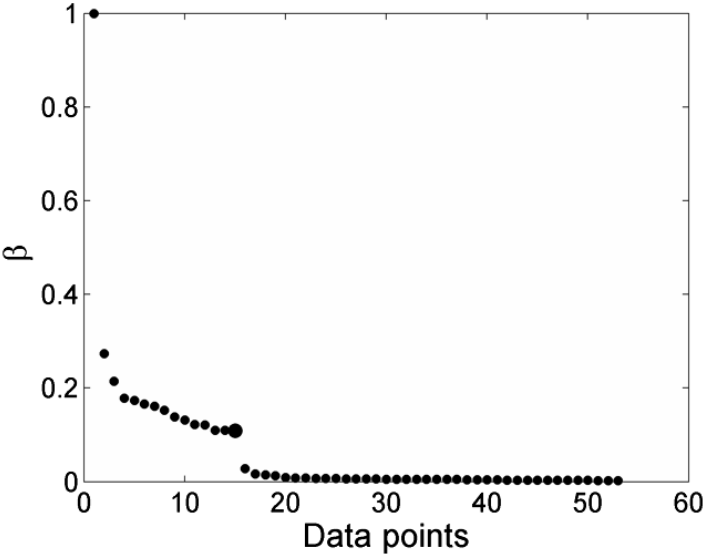
\includegraphics[scale=.15]{4d.png}
    }
    \caption{加速密度聚类算法示例. 图~\ref{sub@fig:4a} 中的白色圆圈和白色星号分别是密度聚类和加速密度聚类结果的聚类中心. 图~\ref{sub@fig:4d} 中较大的圆点代表聚类中心的决策点. }
\end{figure}
如图~\ref{fig:4a} 所示. 二维的``S"型数据集的在空间分布上十分复杂, 它有15个人为设置的聚类中心. 从图~\ref{fig:4a} 中可以看到, 数据点具有非球形的分布, 且不同聚类中心所属的概率分布重叠较为严重. 其中, 白色圆圈是密度聚类算法确定的聚类中心, 白色星号是由加速密度聚类算法确定的聚类中心. 显然, 加速密度聚类算法计算出的聚类中心与原始密度聚类算法计算出的聚类中心完全吻合. 这表明加速密度聚类可以找到与原始密度聚类相同的极大似然解. 图~\ref{fig:4b} 显示了直方图函数所估计出的局部密度, 二维直方图上的密度峰值点保留了中心信息,  而且通过将直方图的格点作为一个新的数据集, 大大降低了计算成本, 因为新数据集中的点数量很少. 图~\ref{fig:4c} 给出了每个数据点的局部密度$\rho_i$和新数据集中密度较高的点的最小距离$\sigma_i$. 图~\ref{fig:4d} 是使用归并排序(\cite{Satish2010})对$\beta$进行排序的排序结果. 在对$\beta$进行排序后, 选择聚类中心为那些$\beta$相对较大的点. 通常情况下, 聚类中心与其他普通点之间会有一个突变, 利用这一特性, 在排序后的$\beta$上应用梯度算子来检测突变. 在图~\ref{fig:4d} 中, 有突变的点用一个较大的圆点表示. $\beta$值大于或等于这个点的数据点被识别为新数据集的聚类中心. 这些点给出了原始数据集的真实聚类中心的大致位置. 然后对这些聚类中心进行更新, 找到真正的中心. 对于一个由$N$个数据点组成的数据集, 加速密度聚类的计算复杂度为$O(1/K(r_M/r_{clu})^4N^2)$, 其中$K$为聚类中心的数量, $r_M$和$r_{clu}$分别为直方图中组距的平均半径和聚类簇的平均半径. 加速密度聚类算法的详细计算复杂度分析见附录~\ref{Appendix:A}. 而密度聚类算法的计算复杂度为$O(N^2)$. 加速密度聚类算法比原密度聚类算法快$K(r_{clu}/r_M)^4$倍. 在`S"型数据集的例子中, 有$5000$个数据点, 在Matlab中编写的新算法在单核CPU上的运行时间为0.3 s, 而原密度聚类算法的运行时间为22 s, 加速后的密度聚类算法速度约原来的为73倍. 

为了更加完整地表示算法的性能, 我们给出了原始数据点的分配结果. 
\begin{figure}[htb]
    \centering
    \subfigure[加速密度聚类算法的分配结果. \label{fig:5a}]{
        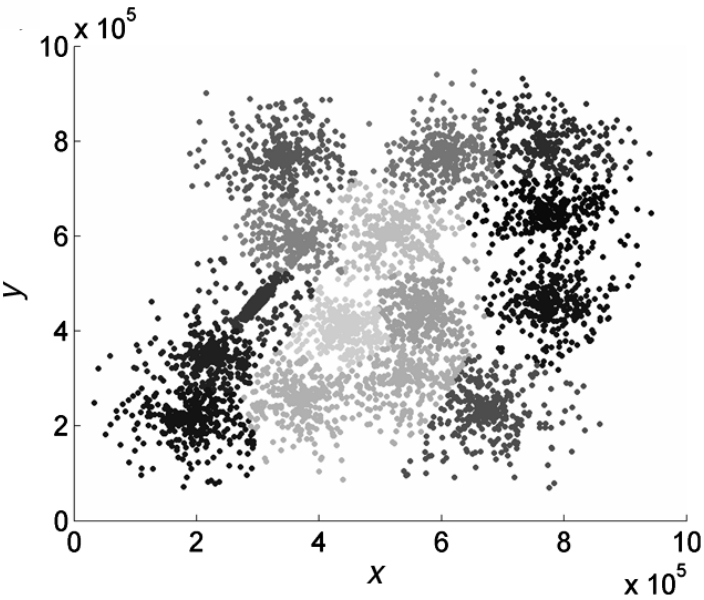
\includegraphics[scale=.15]{5a.png}
    }
    \subfigure[原始密度聚类算法的分配结果. \label{fig:5b}]{
        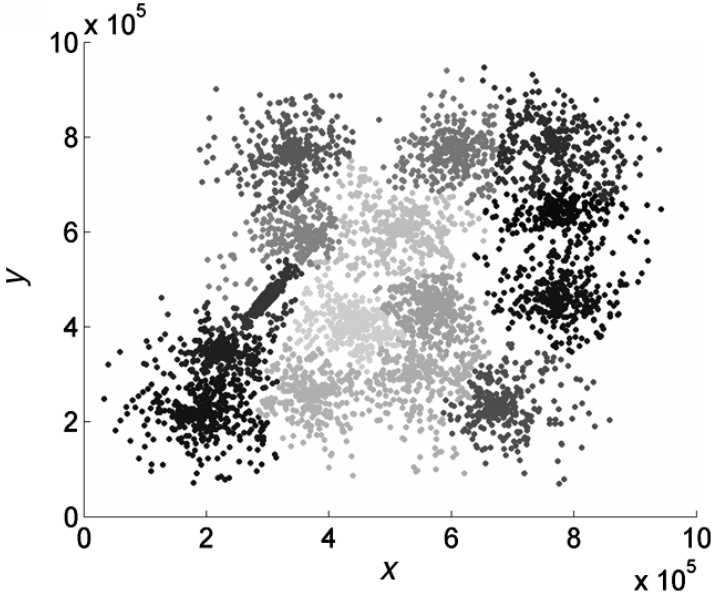
\includegraphics[scale=.15]{5b.png}
    }
    \caption{``S"型数据中数据点的分配结果. 不同灰度表示不同簇. \label{fig:5}}
\end{figure}
图~\ref{fig:5a} 和图~\ref{fig:5a} 分别是我们的算法和原始密度聚类算法的结果. 除了在组的边界处有细微的差异外, 它们的结果十分相似, 这也证明了我们的算法良好性能. 

\subsection{自动速度估计}
通过混合分布模型和加速密度聚类算法的介绍, 我们可以有效地从主要地下构造的同相轴局部斜率中计算出极大似然速度. 同时, 又因为主要的反射体通常具有较高的信噪比, 可以很好地被PWD捕获. 通过计算单个CMP道集的映射后的叠加速度$V_{\mathrm{NMO}}(\tau_0)$和零偏距走时$\tau_0$的聚类中心, 我们可以得到作为结点速度的主反射体速度. 在所有CMP道集上重复这一过程后, 我们就得到了整个测量的结点速度. 因为我们假设叠加速度是横向连续的, 所以从相邻CMP道集点映射得到的局部属性可以添加到当前位置作为聚类的输入. 

将自动叠加速度估计扩展到时偏移速度分析上是很直观的. 只需要将数据从迭前空间$\{t,h,y\}$映射到时偏移图像空间$\{\tau.x.V_{\mathrm{mig}}\}$(\cite{Fomel2007})即可, 其中$y$为中点坐标, $\tau$为时偏移双向垂直走时, $V_{\mathrm{mig}}$为时偏移速度, $x$为时偏移图像坐标. 以映射后的局部属性为输入数据, 对每一个成像点道集(CIG)实施加速密度聚类来提取整个事件的结点时偏移速度. 同样的, 对结果进行插值, 建立时偏移速度模型. 

为了将不均匀采样的聚类后的结点速度插入到格点中, 我们可以通过计算一个插值问题: 
\begin{equation}
    \mathbf{G} \mathbf{v}_{\mathbf {grid }}=\mathbf{v}_{\mathbf{k n o t}}
\end{equation}
其中$v_{\mathrm{grid}}$是规则格点上的速度, $v_{\mathrm{knot}}$取不均匀采样上的结点速度, $G$代表插值算子, 在我们的例子中是立方B-splines插值. 由于我们的目标是建立平稳的时域速度模型, 所以在最小二乘目标函数中加入了一个正则化项$\epsilon$: 
\begin{equation}
\left\|\mathbf{G} \mathbf{v}_{\mathbf {grid }}-\mathbf{v}_{\mathbf{k n o t}}\right\|_{2}^{2}+\varepsilon^{2}\left\|\mathbf{L} \mathbf{v}_{\mathbf{g r i d}}\right\|_{2}^{2}
\end{equation}
其中L代表一个粗化算子(如Laplacian算子). 目标函数的最小化结果为: 
\begin{equation}
    \mathbf{v}_{\mathbf{g r i d}}=\left(\mathbf{G}^{T} \mathbf{G}+\varepsilon^{2} \mathbf{L}^{T} \mathbf{L}\right)^{-1} \mathbf{G}^{T} \mathbf{v}_{\mathbf{k n o t}}
\end{equation}

通过上述公式, 我们建立了规则格点上的速度模型. 这个时域速度模型可以进一步用于时域成像任务. 


    为了测试此算法, 我们首先考虑图~\ref{fig:2}~中的例子, 其数据是从一个具有非球形和剧烈重叠的概率分布中抽取的(图~\ref{fig:2a})。图~\ref{fig:2b}、\ref{sub@fig:2c}~是, 分别从图~\ref{fig:2a}~中中抽取的4000和1000个点, 在相应的决策图(图~\ref{fig:2d}, \ref{sub@fig:2e})中, 只看到5个点的$\sigma$值很大, 密度也相当大。这些点在图中表示为大的实心圆, 对应于聚类中心。选定聚类中心后, 每个点要么被分配到一个簇, 要么被分配到环, 即使是对那些密度非常不同的(图~\ref{fig:2c}~中的蓝色和浅绿色点)和非球形峰, 该算法也可以捕捉到概率分布的位置和形状。此外, 通过目测图~\ref{fig:2a}~中的概率分布可以知道, 分配到环的点对应的区域不会被分到任何类中。

为了表明该算法对大量数据也具有鲁棒性, 我们从图~\ref{fig:2a}~中抽取10000个点进行分析, 将从10000个样本上获得的聚类结果作为参考, 通过只保留一部分点来获得缩小的样本, 并对每个缩小的样本独立地进行聚类。图~\ref{fig:2f}~是分配到一个簇的点的误分率与样本量的关系图像, 可以看到, 即使对只包含1000个点的小样本, 被错误分类的点占比仍然远低于$1\%$。

对图~\ref{fig:2b}~中的数据改变$d_c$, 会产生一致的结果(图~S1 所示\footnote{类似于图~S1, S2~的此类图片可以在\url{http://science.sciencemag.org/content/suppl/2014/06/25/344.6191.1492.DC1}中获得。})。
可以经验地按照如下规律选择$d_c$, 使平均邻域数约为数据量的$1\sim2\%$。对于由少量点组成的数据集, $\rho_i$可能会受到较大的统计误差的影响。在这些情况下, 最好用更精确的方法估计密度\cite{Fukunaga1975,Cheng1995}。
\begin{figure}[ht]
    \centering
    \subfigure[\citeauthor{Gionis2007}(\citeyear{Gionis2007})中的测试结果。\label{fig:3a}]{
        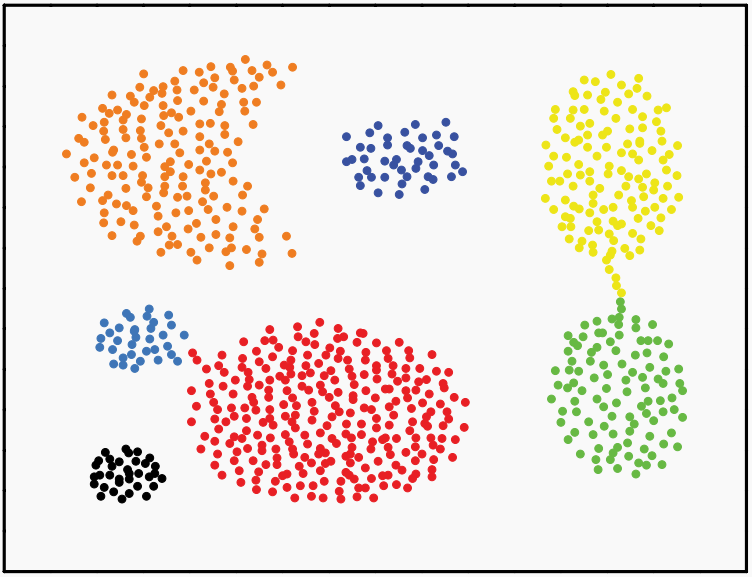
\includegraphics[scale=.2]{3_a.png}
    }\ 
    \subfigure[\citeauthor{Fraenti2006}(\citeyear{Fraenti2006})中的测试结果。\label{fig:3b}]{
        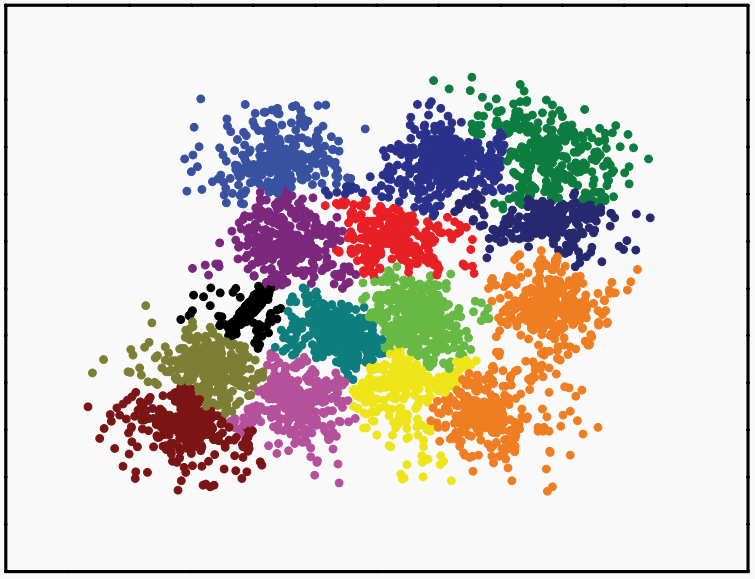
\includegraphics[scale=.2]{3_b.png}
    }\\
    \subfigure[\citeauthor{Fu2007}(\citeyear{Fu2007})中的测试结果。\label{fig:3c}]{
        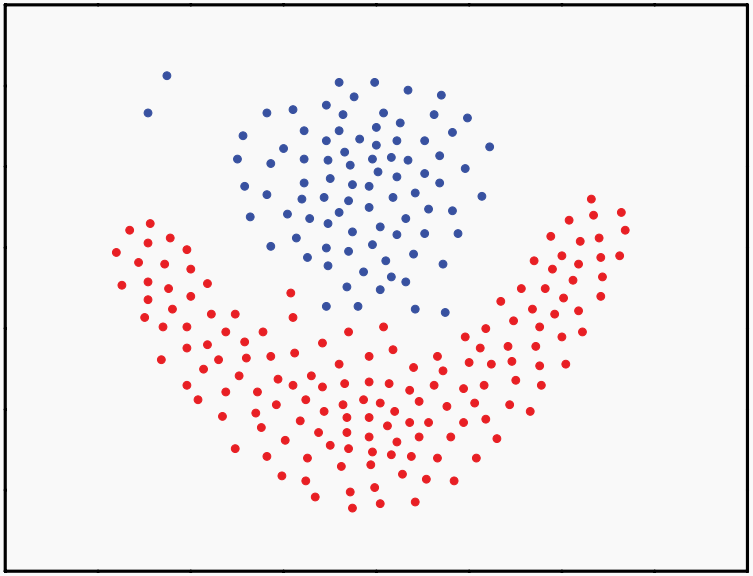
\includegraphics[scale=.2]{3_c.png}
    }\ 
    \subfigure[\citeauthor{Chang2008}(\citeyear{Chang2008})中的测试结果。\label{fig:3d}]{
        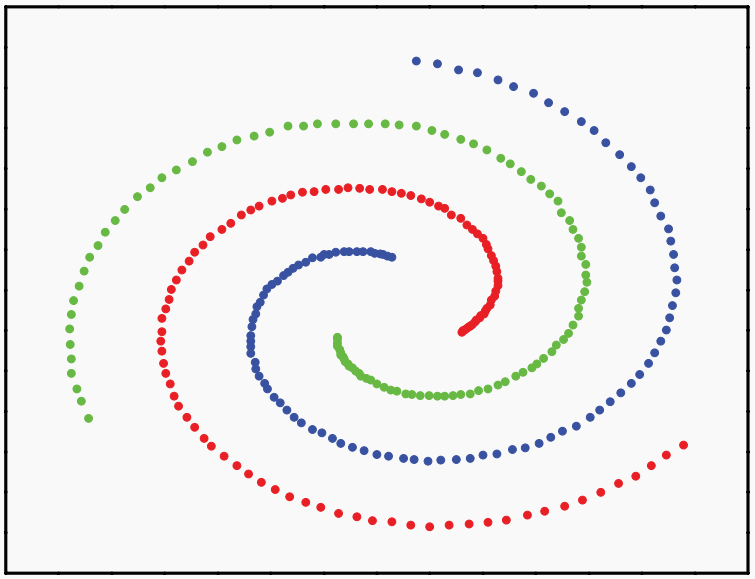
\includegraphics[scale=.2]{3_d.png}
    }
    \caption{其他文献中测试例子的结果。\label{fig:3}}
\end{figure}

接下来, 我们在图~\ref{fig:3}~的例子上对算法进行了测试。对于计算点少的密度, 我们采用了\citeauthor{Cheng1995}(\citeyear{Cheng1995})中描述的指数核算法, 在图~\ref{fig:3a}~中, 我们使用了\citeauthor{Gionis2007}(\citeyear{Gionis2007})中的一个数据集, 得到的结果与原文的结果基本一致, 而文中说到许多常用的方法无法成功将此数据集聚类。在图~\ref{fig:3b}~中, 我们使用了\citeauthor{Fraenti2006}(\citeyear{Fraenti2006})中的一个15个概率分布高度重合的例子, 我们的算法成功地确定了每个簇的结构。在图~\ref{fig:3c}~中, 我们使用了FLAME方法\cite{Fu2007}中的例子, 得到的结果与原始方法高度一致。在图~\ref{fig:4d}~所示的为了说明基于路径的谱聚类\cite{Chang2008}的性能而引入的数据集中, 我们的算法在不需要生成连接图的情况下, 正确地找到了三个簇。作为比较, 在图~S3 和 S4 中, 我们展示了基于路径的谱聚类\cite{Chang2008}的性能。图~S3和 S4 中, 我们展示了这四个测试案例和图~\ref{fig:2}~中的例子通过K-means\cite{MacQueen1967}获得的聚类结果。在大多数情况下, 即使使用正确的K值进行K-means聚类, 也不能得到很好的结果。

该方法对于度量的变化是稳健的, 即保持式~\ref{equ:1}~中的密度估计不变, 这些变化也不会对小于$d_c$的距离产生显著影响。显然, 式~\ref{equ:2}~中的距离会受到这种度量变化的影响, 但决策图的结构(特别是d值大的数据点的数量)是密度值排序的结果, 而不是远处的点之间实际距离的结果, 证明这一说法的例子如图~S5 所示。

我们的方法只需要测量(或计算)所有数据点之间的距离, 而不需要对概率分布\cite{McLachlan2007}或多维密度函数\cite{Fukunaga1975}进行参数化。因此, 其性能不受数据点所嵌入的空间的内在维度影响。同时, 我们还验证了在256个维度\cite{Franti2006}的16个聚类的例子中, 该算法可以找到正确的聚类中心的数量, 并正确的将数据点划分到每一个簇中(图~S6)。对于\cite{Charytanowicz2010}中三类小麦种子的7个X射线特征的210个测量数据, 该算法正确预测了3个簇的存在, 并对$97\%$的数据进行了正确分类(图~S7, S8)。

\begin{figure}[ht]
    \centering
    \subfigure[数据库中前一百张图片的决策图\cite{Samaria1994}。\label{fig:4a}]{
        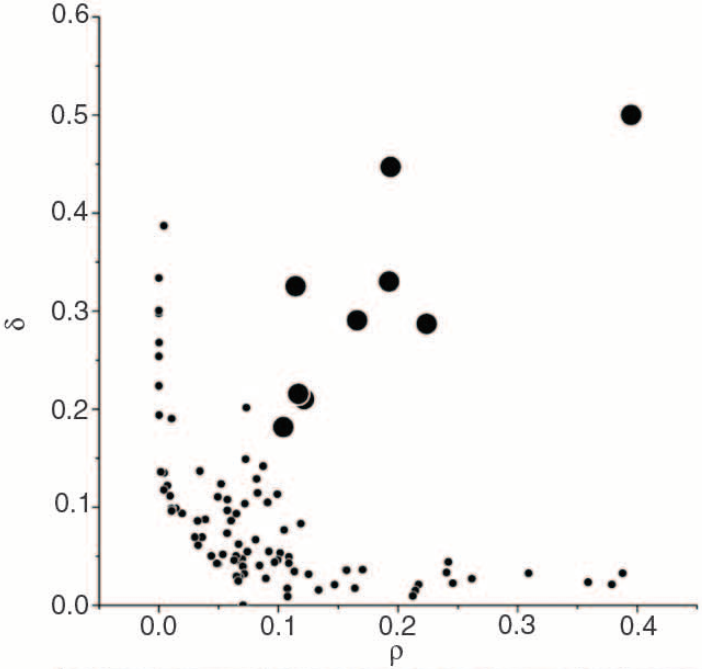
\includegraphics[scale=.18]{4_a.png}
    }\ 
    \subfigure[$\gamma_i=\rho_i\sigma_i$, 其值依次递减。\label{fig:4b}]{
        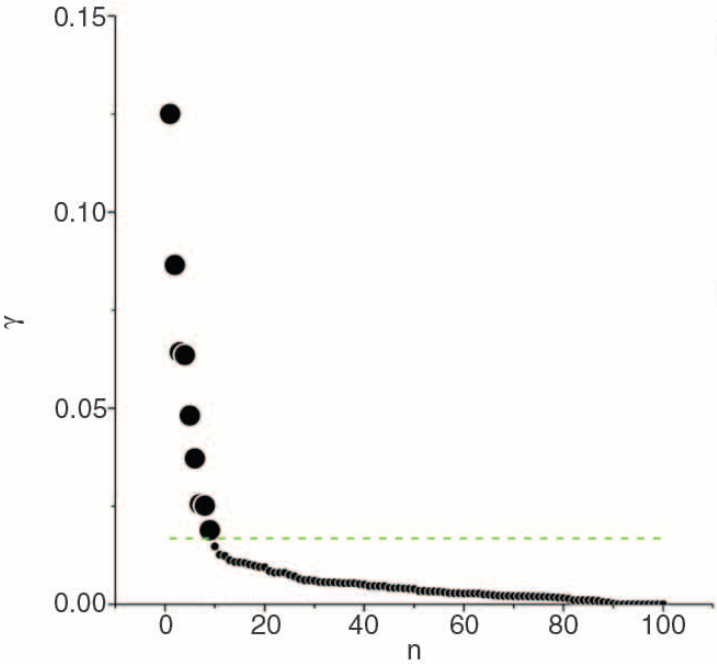
\includegraphics[scale=.18]{4_b.png}
    }\ 
    \subfigure[性能曲线。\label{fig:4c}]{
        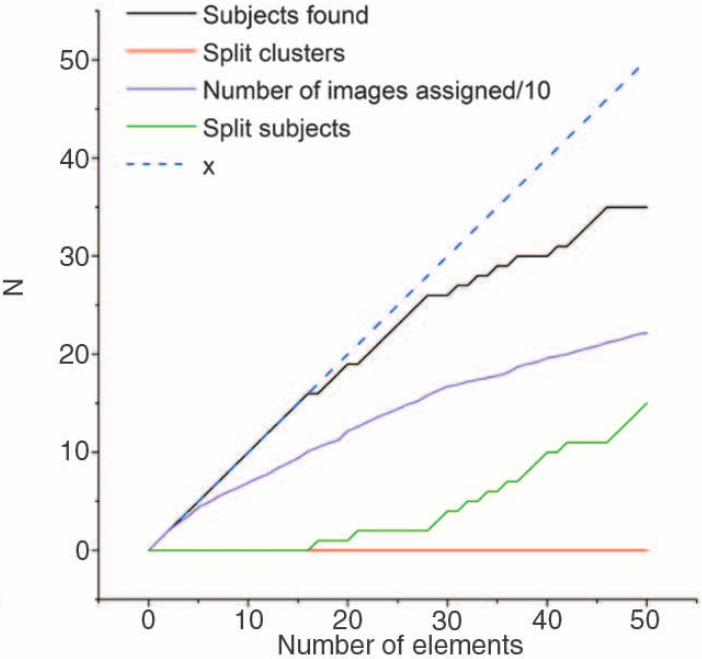
\includegraphics[scale=.18]{4_c.png}
    }\\
    \subfigure[前100张图像的聚类结果的图示。具有相同颜色的面孔属于同一簇, 聚类中心用白色圆圈标注。 \label{fig:4d}]{
        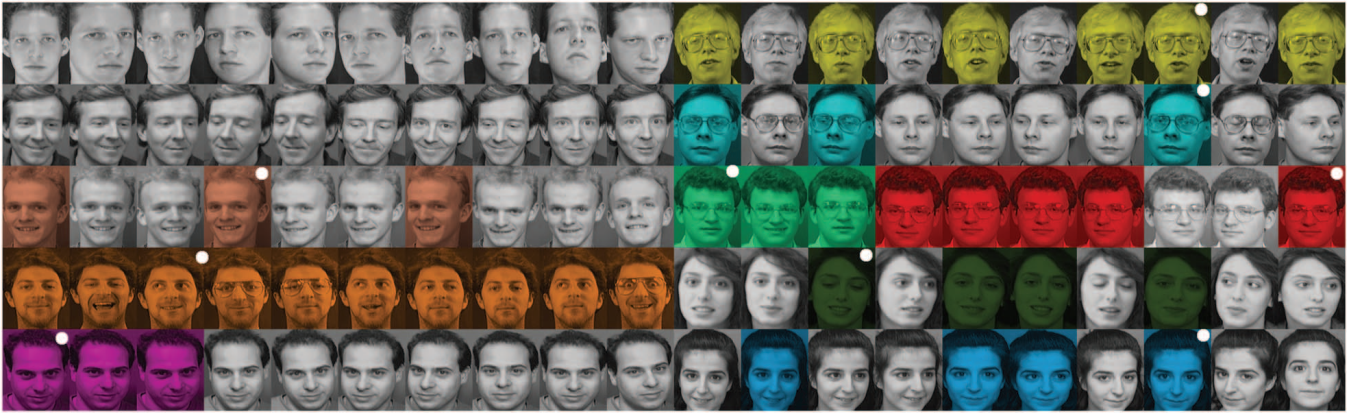
\includegraphics[scale=.30]{4_d.png}
    }
    \caption{Olivetti人脸数据库上的聚类分析。\ref{sub@fig:4c}~中, 黑线是被识别为人像的数量, 红线是包含超过一个人像的簇数, 绿线是在簇中分裂的人物数量, 紫线是划分给一个簇的图像数量除以10。\label{fig:4}}
\end{figure}

我们还将该方法应用于Olivetti人脸数据库\cite{Samaria1994}, 这是机器学习算法的一个较为普遍的测试数据及, 使用这个数据集的目的是在没有任何先前训练的情况下, 希望算法能够识别数据中的不同的人的数量。这个数据集对我们的方法提出了严峻的挑战, 因为``理想"的聚类中心数量与数据集中的样本数量相同, 这使得对密度的估计变得困难。两幅图像之间的相似度是通过\cite{Sampat2009}中的方法计算的, 密度是由一个方差为$d_c=0.07$的高斯核\cite{Cheng1995}估计出来的。对于这样一个小的集合, 密度估计器不可避免地会产生较大的误差, 因此, 我们对于数据点的划分应该更严格一些。只有当一个图像的距离小于$d_c$时, 它才会被分配到与其最近的密度较高的图像的同一簇中。因此, 距离任何其他密度较高的图像比dc更远的图像会不被分配。在图~\ref{fig:4}~中, 我们显示了对数据集中前100张图像进行分析的结果。决策图(图~\ref{fig:4a})显示了几个不同的密度最大值的存在。与其他例子不同的是, 它们的确切数量并不清楚, 这是因为数据比较稀疏性的结果, 按递减顺序排列的$\gamma_i = \rho_i\sigma_i$图提供了一个选择聚类中心数量的提示(图~\ref{fig:4b}), 这张图显示, 聚类中心的数量比较多, 从第九个数据点开始异常增长, 因此, 我们使用9个聚类中心来进行分析。在图~\ref{fig:4d}~中, 我们用不同的颜色显示了这些中心对应的聚类。7个类对应不同的主体, 表明算法能够 ``识别"10个人物中的7个, 第8个被划分到了两个不同的类中。当对数据中的所有400张图像进行分析时, 决策图不能清楚地识别出聚类的数量(图~S9)。然而, 在图~\ref{fig:4c}~中, 可以看出通过增加聚类中心, 大约有30个人物可以被毫不含糊地识别出来(图~S9), 当加入更多的中心时, 一些人物的图像会被划分到两个簇内, 但所有的簇仍然是一致的, 即只包括同一人物的图像。按照\citeauthor{Dueck2007}(\citeyear{Dueck2007})的方法, 我们还计算了同一人物的图像被正确划分到同一簇的比率($r_{\mathrm{true}}$)和不同人物的图像被错误地分配到同一簇的比率($r_{\mathrm{false}}$)。如果在划分中不应用$d_c$处的截止值(即应用我们算法的一般公式), 则在约42到约50个中心的情况下, 可以得到$r_{\mathrm{true}}\sim 68\%$和$r_{\mathrm{false}}\sim 1.2\%$, 这一性能与无监督图像分类的最先进方法相当\cite{Dueck2007}。

最后, 我们对聚类算法进行了基准分析, 在300K的水\cite{Marinelli2009}中对三丙氨酸的分子动力学轨迹进行了分析, 这种情况下, 聚类将近似对应于动力学盆地, 即长时间上稳定的和且被自由能量壁垒隔绝的系统独立构象, 只有在微观时间尺度上偶尔跨越。我们首先通过标准方法\cite{Horenko2006}, 基于动力学矩阵的谱分析对轨迹进行了分析, 其矩阵特征值与系统的松弛时间有关。在第七个特征值(图~S10)之后存在一个空隙, 表明该系统有八个盆地, 与此相一致, 我们的聚类分析(图~S10)也产生了八个聚类, 这与动力学盆地的构象一一对应\cite{Horenko2006}。

识别具有密度最大值的聚类是一个简单而直观的选择, 就像这里和其它基于密度的聚类算法\cite{Ester1996,Fukunaga1975}所做的那样, 但这种方法有一个重要的缺点, 如果随机生成数据点, 那么对于有限样本量所估计的密度远远不是均匀的, 而是以几个最大值为特征。然而, 决策图允许我们将真正的聚类与噪声产生的密度波纹区分开来。定量来看, 只有在前一种情况下, 对应于聚类中心的点与其它点在$\rho$和$\sigma$上有相当大的差距, 对于随机分布, 人们反而会观察到$\rho$和$\sigma$的连续分布。事实上, 我们对超立方体中的均匀分布随机生成的点进行了分析, 在式~\ref{equ:1}~和~\ref{equ:2}~的点之间的距离是在超立方体上的周期性边界条件下计算出来的, 这一分析表明, 对于随机分布的数据点, 数量$\gamma_i= \rho_i\sigma_i$是按照幂律分布的, 其指数取决于点所在空间的维度。对于实际的数据集, 如图~\ref{fig:2}~至图~\ref{fig:4}~中的数据集, $\gamma$的分布与幂律有明显的不同, 特别是在高$\gamma$的区域(图~S11)上。这一结果可以为自动选择聚类中心的提供标准以及在统计学上对我们的算法的验证的可靠性提供依据。




    \appendix

    \printbibliography

\end{document}